\chapter{Alternative Models for the Encounter Process}
\label{chapt.poisson-mn}

In the previous chapter we considered a very specific but not
terribly limited observation model. The observation model consisted of
two main elements: First a description of the encounter process
by which individuals are detected in traps. Specifically, we
assumed individual trap-specific encounters were iid Bernoulli
trials. The consequence of this is that individuals function
independently of one another and can be captured in
any number of traps during a specific interval of trapping
effort, but only 1 time per trap. 
The type of device is typical of bear hair snares, which we
considered as an example in that section. 
 It is natural to consider
alternative functional forms of this detection probability model which
we do in Chapt. \ref{chapt.covariates} and elsewhere.

In this chapter we consider alternative observation models which
accommodate Poisson or multinomial observation models. For example, if
sampling devices can detect an individual some arbitrary number of
times during an interval, then it is natural to consider observation
models for encounter frequencies, such as the Poisson model. Another
type of encounter device is the ``multi-catch'' device
\citep{efford_etal:2009euring} which
is a physical device that can capture and hold an arbitrary number of
individuals. A typical example is a mist-net for birds
\citep{borchers_efford:2008}.  It is natural to regard observations
from these kinds of studies as independent multinomial observations.
A related type of device that produces {\it dependent} multinomial
observations are the so-called {\it single-catch} traps
\citep{efford_etal:2009euring}. The canonical example are small-mammal
live traps which catch and hold a single individual. Competitation
among individuals for traps induces a complex dependence structure
among individual encounters. To date, no formal inference framework
has been devised for this method although it stands to reason that the
independent multinomial model should be a good approximation in some
situations \citep{efford_etal:2009euring}.  There are other
observation systems that we discuss here.

One thing that is apparent from our development of the multinomial
observation model is that SCR models are a kind of multi-state model,
in the conventional sense as applied in capture-recapture studies. In
the context of SCR though, the ``state'' variable is a geographic
location and the transition probabilities are parameterized by
distance between the states.





\section{Poisson Observation Model}

The models we analyze in Chapt. \ref{chapt.scr0} assumed binary
observations -- i.e., standard encounter history data -- so
that individuals are captured at most one time in a trap.  This makes
sense for many types of DNA sampling (e.g., based on hair snares)
because distinct visits to sampled locations or devices cannot be
differentiated. However, many encounter methods or devices make it
possible to encounter an individual some arbitrary number of times
during any particular sampling episode XXXX EFFORD CITE XXXXXX. 
That is, we might observe
encounter frequencies $y_{ijk}>1$
for individual $i$, trap $j$ and
sampling interval $k$.  As an example, if a camera device is
functioning properly it may be programmed to take photos every few
seconds if triggered.  For a second example, suppose we are searching
a quadrat or length of trail for scat, we may find multiple samples from the same
individual.
Therefore, we seek observation models that accommodate such encounter
frequency data.  In general, any discrete probability mass function
could be used for this purpose, including the standard models for
count data used throughout ecology, the Poisson and negative
binomial.  Here we focus on using the Poisson
model only although other count frequency models are possible XXX
EFFORD ciTE XXXX.

Let $y_{ijk}$ be the frequency of encounter for
individual $i$, in trap $j$, during occasion $k$, then assume:
\[
 y_{ijk} \sim \mbox{Poisson}(\lambda_{ij})
\]
where the expected encounter frequency $\lambda_{ij}$ depends on both
individual and trap. As we did in the binary model of
Chapt. \ref{chapt.scr0}, we
now seek to model the expected value of the observation (which was
$p_{ij}$ in Chapt \ref{chapt.scr0}) as a function of the individual activity center
${\bf s}_{i}$.
We propose
\[
 \lambda_{ij} = \lambda_{0}  g({\bf x}_{j},{\bf s}_{i})
\]
Where $g({\bf x},{\bf s})$ is any positive valued function, such as
the negative exponential or the bivariate Gaussian kernel.
Then $\lambda_{0}g({\bf x},{\bf s})$ is the expected encounter rate in trap
${\bf x}$ for an individual having activity center ${\bf s}$.  Note
that
\[
 log(\lambda_{ij}) = log(\lambda_{0}) + log(  g({\bf x}_{j},{\bf
   s}_{i}) )
\]
where, if we set $\alpha_{0} \equiv log(\lambda_{0})$, and, if 
$g({\bf x},{\bf s}) \equiv exp(-\alpha_{1} d({\bf x},{\bf s})^2)$
(i.e., the Gaussian model), then:
\begin{equation}
 log(\lambda_{ij}) = \alpha_{0} + \alpha_{1} d({\bf x}_{j},{\bf s}_{i})^{2}
\label{poisson-mn.eq.lp}
\end{equation}
which is the same linear predictor as we have seen for the Bernoulli
model in Chapt. \ref{chapt.scr0}.  We can accommodate covariates at
the level of individual-, trap- or sample occasion by including them
on the baseline encounter rate parameter $\lambda_{0}$. For example,
if $C_{j}$ is some covariate that depends on trap only, then we have:
\[
log(\lambda_{0,ijk}) = \alpha_{0} + \alpha_{2} C_{j}
\]
and therefore covariates on the logarithm of baseline encounter
probability appear also as linear effects on $\lambda_{ij}$.  We don't
get into too much discussion of general covariate models here, but see
Chapt. \ref{chapt.covariates} for a more comprehensive development of
such models along with examples. 


For a  model in which we have covariates that vary across
the sample occasions  $k$, we can aggregate the observed data by the
property of compound additivity of the Poisson distribution (if $x$ and
$y$ are $iid$ Poisson with mean $\lambda$ then $x+y$ is Poisson with
mean $2\lambda$). Therefore,
\[
y_{ij} = (\sum_{k=1}^{K} y_{ijk}) =  \mbox{Poisson}(K  \lambda_{0}
g({\bf x}_{j},{\bf s}_{i}) )
\]
We see that $K$ and $\lambda_{0}$ serve the same role as affecting the
base encounter rate. Since the observation model is the same,
probabilistically speaking, for all values of $K$, evidently we need
only $K=1$ ``survey'' from which to estimate model parameters. We know
this intuitively as sampling by multiple traps serves as replication
in SCR models.

\subsection{Poisson model of space usage}

How do we interpret this model?  A natural interpretation of the
encounter process model is that resulting from movement of individuals
about their home range (sec. \ref{scr0.sec.implied}).  Imagine we have
perfect samplers in every pixel of the landscape that discharge at set
time intervals (e.g., every hour), and let $m_{ij}$ be the number of
times individual $i$ was recorded in pixel $j$. For pure model of
space usage, we might think of this model:
\[
m_{ij} \sim  \mbox{Poisson}(K  g({\bf x}_{j},{\bf s}_{i}) )
\]
where $K$ is the number of time intervals recorded. This model of
space usage gives rise to the standard resource selection function
(RSF) models \citep[][and Chapt. \ref{chapt.rsf}]{royle_etal:2012mee}.
But now suppose our samplers are not perfect but, rather, record only
a fraction of the resulting visits. A sensible model is
\[
 y_{ij}|m_{ij} \sim \mbox{Bin}(m_{ij}, \lambda_{0}).
\]
The marginal distribution of $y_{ij}$ is:
\[
 y_{ij} \sim \mbox{Poisson}(K \lambda_{0} g({\bf x}_{j},{\bf s}_{i}) ).
\]
Therefore, we see that encounters accumulate in proportion to the
frequency of outcomes of an individual using space (or ``selecting
resources'').

We introduced this interpretation of the model in terms of movement
and space usage in sec. \ref{scr0.sec.implied}, and it is one of the
main underlying concepts of SCR models that is not present in ordinary
capture-recapture models. As we noted previously, the underlying model
of space usage is only as complex as the encounter probability (or
rate) model which is, so far, only symmetric and stationary (does not
vary in space). 




\subsection{Poisson relationship to the Bernoulli model}
\label{poisson-mn.sec.approx}

There is a sense in which the Poisson and Bernoulli models can
be viewed as consistent with one another. Note that under the Poisson
model with $E(y) = \lambda$ we have:
\begin{equation}
 \Pr(y>0) = 1-exp(-\lambda)
\label{eq.cloglog}
\end{equation}
Therefore, if we equate the event ``encountered'' with the event that
the individual was captured at least 1 time under the Poisson model,
i.e., $y>0$, then it would be natural to set $p_{ij} = \Pr(y>0)$
according to \ref{eq.cloglog}.

In fact, as $\lambda$ gets small, the Poisson model is a close approximation
to the Bernoulli model in the sense that outcomes concentrate on
$\{0,1\}$, i.e.,  $\Pr(y\in \{0,1\})
\rightarrow 1$ as $\lambda \rightarrow 0$.
A relevent property of the Poisson model
is that
$\Pr(y>0) \rightarrow \lambda$
for small values of $\lambda$.
This phenomenon is shown in  Fig.
\ref{poisson-mn.fig.poissonbern} where
the left panel shows a plot of $\lambda_{ij}=\lambda_{0}g({\bf
  x}_{j},{\bf s}_{i};\sigma)$ vs. distance and
superimposed on that is a plot of $p_{ij}=1-exp(-\lambda_{ij})$ vs. distance, for values
$\lambda_{0} = .1$ and $\sigma = 1$, and the right panel shows a plot of
$\Pr(y>0)$ vs. $E[y]$. We see that the two quantities are
practically indistinguishable.

This is
convenient in some cases because the Poisson model might be more
tractable to fit (or even vice versa). For an example, see the models
described in Chapt. \ref{chapt.scr-unmarked}, and we also consider
another case in sec. \ref{poisson-mn.sec.singlecatch} below. To
evaluate the closeness of the approximation, you can use the following
{\bf R} commands which we used to produce
Fig. \ref{poisson-mn.fig.poissonbern}:
{\small
\begin{verbatim}
x<-seq(0.001,5,,200)
lam0<- .1
sigma<- 1
lam<- lam0*exp(-x*x/(2*sigma*sigma))

par(mfrow=c(1,2))
p1<- 1-exp(-lam)
plot(x,lam,ylab="E[y] or Pr(y>0)",xlab="distance",type="l",lwd=2)
lines(x,p1,lwd=2,col="red")
plot(lam,p1,xlab="E[y]",ylab="Pr(y>0)",type="l",lwd=2)
abline(0,1,col="red")
\end{verbatim}
}

To summarize, if $y$ is Poisson and, as $\lambda$ gets small,
\begin{eqnarray*}
\Pr(y>0)  & \approx & E[y]  \\
1-exp(-\lambda_{0} g(x,s)) &\approx &  \lambda_{0} g(x,s)
\end{eqnarray*}
which explains the close correspondance we have found between these
two versions of the Gaussian encounter probability model (sec. \ref{scr0.sec.implied}).
What all of this suggests it that
if we see very few observations $>1$ then we wont lose much
information by using the Bernoulli model. On the other hand, the
Poisson model may have some advantages in terms of analytic or numerical
tractability in some cases.

\begin{figure}
\centering
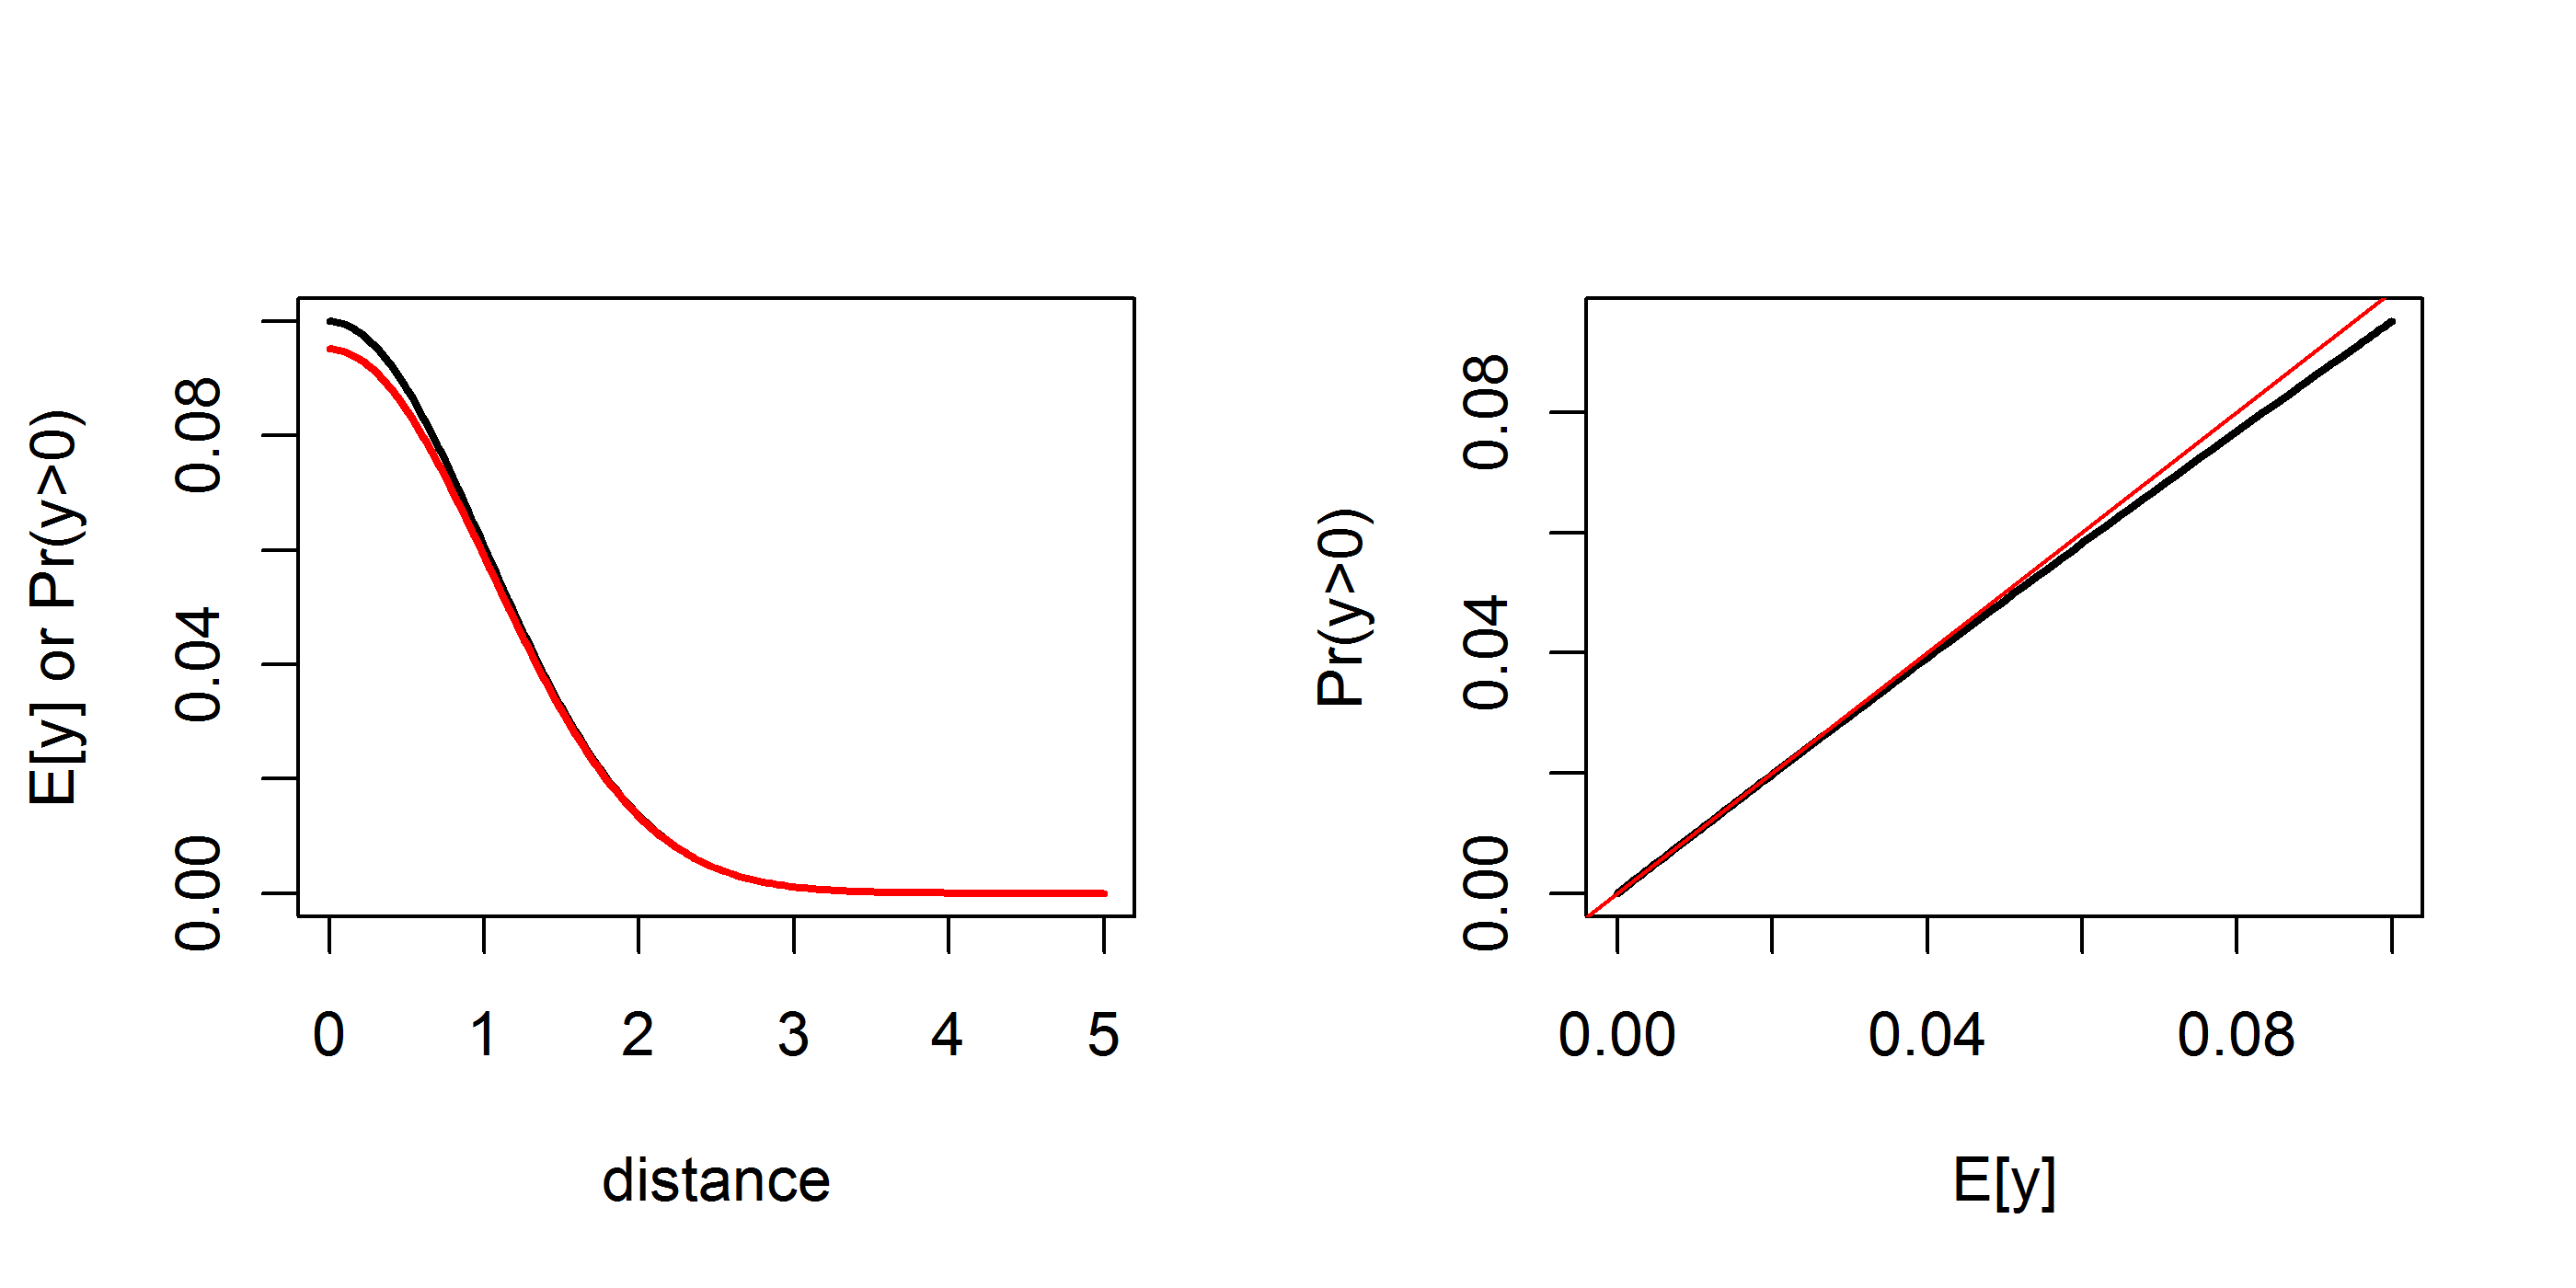
\includegraphics[width=5in,height=2.5in]{Ch5-PoisMn/figs/Poisson-Bern.png}
\caption{Poisson approximation to the binomial. As the Poisson mean
  approaches 0, then $Pr(y>0)$ under the Poisson model approaches
  $\lambda$ and therefore $y \sim Poisson$ is well-approximated by a
  Bernoulli model with parameter $\lambda$.
}
\label{poisson-mn.fig.poissonbern}
\end{figure}

Even in such cases where we're not in the range where the Poisson and
Bernoulli models are nearly equivalent,
we might choose to truncate  individual encounter frequencies
to binary observations anyhow (``quantize'').
We might do
this intentionally, but sometimes this truncation is a feature of the
sampling. For example, in the case of bear hair snares, the number of
encounters might be well approximated by a Poisson distribution but we
cannot determine unique visits and so only get to observe the binary
event ``$y>0$''. Similarly for scat sampling problems it will not
generally be possible to diagnose distinct ``independent'' scat
samples. Under this model the data are only binary encounters and we
might therefore choose a model of the form:
\[
\mbox{ cloglog}(p_{ij}) = \log(\lambda0)  + \log(g({\bf x},{\bf s}))
\]
\begin{comment}
This example shows us that the choice of link function is typically
directly related to a specific encounter frequency model and,
furthermore, the choice of link function is equivalent to choice of
``detection function.''
%As another example, what if the latent
%encounter frequencies are actually geometric random variables where
%the mean is a function of distance? For the case where the support of
%y includes 0 – so that $y$ is the number of failures before the 1st
%success, then the mean is $\mu = (1-p)/p$.  $Pr(y>0) =$ ??
%\[
%logit() = ….?
%\]
\end{comment}

\subsection{A cautionary note on modeling encounter frequencies}

Other models for counts might be appropriate. For example, ecologists
are especially fond of negative binomial models for count data
\citep{verhoef_boveng:2007,white_bennetts:1996,kery_etal:2005}
but other models for excess-Poisson variation are possible. For
example, we might add a normally distributed random effect to
the linear predictor.

As a general rule we favor the Bernoulli observation model even if
encounter frequencies are obtained by sampling.  The main reason is
that, with frequency data, we are forced to confront a model choice
problem (i.e., Poisson, negative binomial, log-normal mixture) that is
wholly unrelated to the fundamental space usage process that underlies
the genesis of SCR data. Repeated encounters over short time intervals
are not likely to be the result of independent encounter
processes. E.g., an individual moving back and forth in front of a
camera yields a cluster of observations that is not informative about
the spatial structure of the model. Similarly in scat surveys (e.g.,
Thompson et al. in review), dogs are used to locate scats which are
processed in the lab for individuality.  The process of local scat
deposition is not really the outcome of movement or space usage but rather the
outcome of complex behavioral considerations as well as dependence in
detection of scat by dogs. E.g., they find one and then more likely to
find a nearby one, or they get into a den area and find lots of scats.
This additional model assumption required to model variation in
observed frequencies (i.e., conditional on location) provides
relatively no information about density, and we feel that the
model selection issue should therefore be avoided.

To elaborate on this, it seems natural to construct models for
encounter data that are conditional on movement outcomes: We suppose
that an individual visits a particular pixel ${\bf x}$ with some probability
$p({\bf x}, {\bf s})$,
 and then, once its
there, deposits a
number of scat, or visits a camera some number of times with frequency
$y(x,s) \ge 0$.
We describe the outcome of this movement/usage with
a two-level hierarchical model of the form:
$[y|z][z|p({\bf x},{\bf s})]$.
Let $z({\bf x},{\bf s})$ be a binary variable
that indicates whether the individual with activity center ${\bf s}$
visits pixel ${\bf x}$ during some interval, and let
$z({\bf x},{\bf s}) \sim  \mbox{Bern}(p({\bf x},{\bf s}))$ and
suppose
 the encounter frequency $y$ is independent of ${\bf x}$ and
${\bf s}$ conditional
on the binary event $z$,  that the individual visited pixel $x$.
Therefore, the model for $y$ (amount of use) does not
depend on ${\bf s}$.

\begin{comment}
Moreover, consideration of encounter frequency data could lead to
important identifiability problems along the lines of \citet{link:2003}. The
basic Poisson model can be over-dispersed in a number of ways to
produce different models of over-dispersion.  i.e., gamma noise,
normal noise, exponential noise, etc..  Thus we have different models
of heterogeneity, analogous to the class of models considered by
\citet{link:2003},
\end{comment}

\section{Analysis of the Poisson SCR model in BUGS}

We consider the simplest possible model here in which we have no
covariates that vary over sample occasions  $k=1,2,\ldots,K$ 
so that we work with
the aggregated individual- and trap-specific encounters:
\[
y_{ij} = (\sum_{k=1}^{K} y_{ijk}) =  \mbox{Poisson}(K  \lambda_{ij})
\]
We consider a bivariate normal form of $g({\bf x}_{j},{\bf s}_{i})$ so
that
\[
g({\bf x}_{j},{\bf s}_{i}) = exp( -d({\bf x}_{j}, {\bf
  s}_{i})^{2} /(2\sigma^{2}))
\]
so that 
\[
log( \lambda_{ij})  =\alpha_{0} + \alpha_{1} d({\bf x}_{j}, {\bf s}_{i})^2
\]
where $\alpha_{0} = log(\lambda_{0})$ and $\alpha_1 = 1/(2\sigma^2)$.


As usual, we approach Bayesian analysis of these
models using data augmentation (sec. \ref{closed.sec.da}).
Under data augmentation, we introduce a collection of all-zero encounter
histories to bring the total size of the data set up to $M$, and a corresponding
set of data augmentation variables $z_{i} \sim \mbox{Bern}(\psi)$. Then
the observation model is specified conditional on $z$ according to:
\[
y_{ij} \sim  \mbox{Poisson}(z_{i} K  \lambda_{ij})
\]
which evaluates to a point mass at $y=0$ if $z=0$.  In other words, the
observation model under data augmentation is a zero-inflated Poisson
model which is easily analyzed by Bayesian methods, e.g., in one of
the {\bf BUGS}
dialects, or  using likelihood methods, which we neglect here although
the same principles as in Chapt. \ref{chapt.mle} apply.


\subsection{Simulating Data and Fitting the Model}


Simulating a sample SCR data set under the Poisson model requires only
a couple minor modifications to the procedure we used in
Chapt. \ref{chapt.scr0}. In
particular, we modify the block of code which defines the model to be
that of $E(y)$ and not $\Pr(y=1)$, and we change the random variable
generator from \mbox{\tt rbinom} to \mbox{\tt rpois}:
{\small
\begin{verbatim}
D<- e2dist(S,traplocs)

alpha0<- -2.5
sigma<- 0.5
alpha1<- 1/(2*sigma*sigma)

muy <-  exp(alpha0)*exp(-alpha1*D*D)
# now generate the encounters of every individual in every trap
Y<-matrix(NA,nrow=N,ncol=ntraps)
for(i in 1:nrow(Y)){
 Y[i,]<-rpois(ntraps,K*muy[i,])
}
\end{verbatim}
}

We modified our simulation code from Chapt. \ref{chapt.scr0} to
simulate Poisson encounter frequencies for each trap and then we
analyze an ideal data set using {\bf BUGS}. The new function,
available in the \mbox{\tt scrbook} package, is called {\tt
  simPoissonSCR.fn}.  The simulator can produce 3-d encounter history
data too although we don't do that here.  Here is an example of
simulating a data set and harvesting the required data objects, and
doing the data augmentation:

{\small
\begin{verbatim}
data<-simPoissonSCR.fn(discard0=TRUE,sd=2013)
y<-data$Y
traplocs<-data$traplocs
nind<-nrow(y)
X<-data$traplocs
K<-data$K
J<-nrow(X)
Xl<-data$xlim[1]
Yl<-data$ylim[1]
Xu<-data$xlim[2]
Yu<-data$ylim[2]

## Data augmentation stuff
M<-200
y<-rbind(y,matrix(0,nrow=M-nind,ncol=ncol(y)))
z<-c(rep(1,nind),rep(0,M-nind))
\end{verbatim}
}

The process for fitting
the model in \winbugs  or \jags is identical to what we've done
previously in Chapt. \ref{chapt.scr0}. In particular, we set up some
starting values, package the data and inits, identify the parameters
to be monitored, and then send everything off to our MCMC engine. Here
it all is for fitting the Poisson observation model (these commands
are shown in the help file for \mbox{\tt simPoissonSCR.fn}):

{\small
\begin{verbatim}
sst<-traplocs[sample(1:J,M,replace=TRUE),] # starting values for s
for(i in 1:nind){
if(sum(y[i,])==0) next
sst[i,1]<- mean( X[y[i,]>0,1] )
sst[i,2]<- mean( X[y[i,]>0,2] )
}
sst<-sst + runif(nrow(sst)*2,0,1)/8
data <- list (y=y,X=X,K=K,M=M,J=J,Xl=Xl,Yl=Yl,Xu=Xu,Yu=Yu)
inits <- function(){
  list (alpha0=rnorm(1,-2,.4),alpha1=runif(1,1,2),s=sst,z=z,psi=.5)
}
parameters <- c("alpha0","alpha1","N","D")

cat("
model {
alpha0~dnorm(0,.1)
alpha1~dnorm(0,.1)
psi~dunif(0,1)

for(i in 1:M){
 z[i] ~ dbern(psi)
 s[i,1]~dunif(Xl,Xu)
 s[i,2]~dunif(Yl,Yu)
for(j in 1:J){
d[i,j]<- pow(pow(s[i,1]-X[j,1],2) + pow(s[i,2]-X[j,2],2),0.5)
y[i,j] ~ dpois(lam[i,j])
lam[i,j]<- z[i]*K*exp(alpha0)*exp(- alpha1*d[i,j]*d[i,j])
}
}
N<-sum(z[])
D<- N/64
}
",file = "SCR-Poisson.txt")

nthin<-1; nc<-3; nb<-1000; ni<-2000

library("R2WinBUGS'')
out1 <- bugs (data, inits, parameters, "SCR-Poisson.txt", n.thin=nthin,n.chains=nc,
 n.burnin=nb,n.iter=ni,working.dir=getwd(),debug=TRUE)
\end{verbatim}
}
{\flushleft Or using {\bf JAGS}  we do this instead: }
{\small
\begin{verbatim}
library(rjags)
fm <- jags.model("SCR-Poisson.txt", data=data, inits=inits, n.chains=nc, n.adapt=nb)
out2 <- coda.samples(jm, parameters, n.iter=ni, thin=nthin)
\end{verbatim}
}
{\flushleft 
Summarizing } the output from the {\bf WinBUGS}  run produces the following:
{\small
\begin{verbatim}
> print(out1,digits=2)
Inference for Bugs model at "SCR-Poisson.txt", fit using WinBUGS,
 3 chains, each with 2000 iterations (first 1000 discarded)
 n.sims = 3000 iterations saved
           mean    sd   2.5%    25%    50%    75%  97.5% Rhat n.eff
alpha0    -2.57  0.19  -2.95  -2.69  -2.57  -2.44  -2.19 1.00  2600
alpha1     2.34  0.36   1.69   2.08   2.32   2.57   3.12 1.00  3000
N        114.13 15.25  87.97 103.00 113.00 124.00 147.00 1.01   370
D          1.78  0.24   1.37   1.61   1.77   1.94   2.30 1.01   370
deviance 329.95 21.92 290.00 314.20 329.50 344.40 375.80 1.00  1700

...
[..some output deleted..]
...
\end{verbatim}
}

%We don't provide a real example of a Poisson SCR model here although
%we use this observation model for an analysis of some data in Chapt.
%\ref{chapt.searchencounter}. {\bf XXXX DO WE DO THIS ANYWHERE? XXXXX}

\begin{comment}
\subsection{Exercise}

Use the Bernoulli model simulator from Chapt. \ref{chapt.scr0} (\mbox{\tt
  simSCR0.fn}) to simulate a Bernoulli data set and then fit the
Poisson model. Compare the results of fitting the correct
data-generating model with those of fitting the misspecified Poisson
model.
\end{comment}


\section{Analysis of the Wolverine Study Data}

We reanalyzed the data from
the  wolverine camera trapping study that were first introduced in 
sec. \ref{chapt.scr0.wolverine}.
We modified the {\bf R} script from the function \mbox{\tt wolvSCR0.fn} to fit the
Poisson model (see the help file for \mbox{\tt
  wolvSCR0pois.fn}). Executing this function produces the following
results which are provided here:
{\small
\begin{verbatim}
Inference for Bugs model at "modelfile.txt", fit using WinBUGS,
 3 chains, each with 6000 iterations (first 1000 discarded)
 n.sims = 15000 iterations saved
           mean    sd   2.5%    25%    50%    75%  97.5% Rhat n.eff
psi        0.30  0.07   0.19   0.25   0.30   0.34   0.45    1   650
sigma      0.64  0.06   0.54   0.60   0.64   0.68   0.76    1   730
lam0       0.06  0.01   0.04   0.05   0.06   0.06   0.08    1  5000
logp0     -2.89  0.17  -3.22  -3.00  -2.89  -2.78  -2.57    1  5000
N         60.12 11.91  40.00  52.00  59.00  68.00  87.00    1   630
D          5.80  1.15   3.86   5.01   5.69   6.55   8.39    1   630
beta       1.24  0.21   0.86   1.10   1.23   1.38   1.69    1   730

...
[some output deleted]
...
\end{verbatim}
}
The results are almost indistinguishable from the Bernoulli model
fitted preveiously, where we had a posterior mean for $N$ of
 $59.84$,  $\sigma$ it was
$0.64$. The {\bf R} 
script is provided in the  \mbox{\tt scrbook} package which you can
use to modify the model or obtain more posterior samples for this model.
%In addition we did a basic assessment of Goodness-of-fit using a
%Bayesian p-value and statistic 1 as described in sec. XXXXX.  


\begin{comment}
\section{Likelihood analysis of the Poisson model}

Counts are Poisson with a random effect so this is stupidly easy to
implement.
We do the normal ``full likelihood'' approach in which we retain $N$
as a real parameter in the model. We adapt \mbox{\tt intlik3} from
chapter 5 here..... behold:

Poisson(lambda(s,x))

data augmentation = ZIP
\begin{verbatim}
Pr(yi) =   ( prod_{j} dpois(y) ) *psi + I(y=0)*(1-psi)

Actually if y(i,j) = Poisson( lambda(i,j) ) then we can just add up
sum_{j} y(i,j) =  Poisson( sum_{j} lambda(i,j)) right?

 int_{s} thatthing

Zero-inflate the result
\end{verbatim}
\end{comment}



\section{Independent Multinomial Observations}

Several types of encounter devices yield multinomial observations in
which an individual can be caught in a single trap during a particular
encounter occasion, but traps might catch any number of individuals.
Mist nettting is the canonical example of such a ``multi-catch'' traps
\citep{efford_etal:2009euring}. Also some kinds of bird or mammal
traps hold multiples of animals, and pit-fall traps are commonly used
for many types of herptiles.  Another type of sample method that might
be viewed (in some cases) as a multi-catch device are area-searches
of, for example, reptiles where we think of a small polygon as the
``trap'' -- we could get multiple individuals (turtles, lizards) in
the same plot but not, in the same sample session, at different plots.
The key feature is that capture of an individual in a trap is {\it
  not} independent of capture in other traps, because once they are
captured in a trap, it precludes capture in other traps.  On the other
hand, individuals may behave independently of one another, or so it
might be reasonable to assume, so whether a trap captures some other
individual doesn't have bearning on whether it captures another.  This
last assumption is violated in an extreme case in classical ``single
catch'' traps which we address in
sec. \ref{poisson-mn.sec.singlecatch} below. In general we could
imagine non-independence being important in any multi-catch situation
but to the best of our knowledge a general model that encompasses
complete dependence (i.e., single-catch) and complete independence
(multi-catch) of individuals has not been proposed.  So we treat the
cases individually and, in this section, we address the multi-catch
situation wherein individuals behave independently.


In this case we assume the observation ${\bf y}_{ik}$ for
individual $i$ during sample occasion $k$ as a multinomial observation
which consists of a sequence of 0's and at most a single 1 indiciating
the trap of capture, or ``not captured''. For the ``not captured'' event we define an
additional outcome, by conveniton element $J+1$ of the vector.
As an example, 
 if we capture an individual in trap
2 during a 6 sample period study then the multinomial observation has
length $J+1 = 7$, and the observation is ${\bf y}_{i} =
(0,1,0,0,0,0,0)$. An individual not captured at all would have the
observation vector
$(0,0,0,0,0,0,1)$. 
If we sample for 5 periods in all and the individual is also caught
in trap 4 during sample 3, but otherwise uncaptured, then the 5 encounter observations for that
individual are as follows:
\begin{verbatim}
sample |---- trap ---------|
       1   2   3   4   5   6   7
 1     0   1   0   0   0   0   0
 2     0   0   0   0   0   0   1
 3     0   0   0   1   0   0   0
 4     0   0   0   0   0   0   1
 5     0   0   0   0   0   0   1
\end{verbatim}
Statistically we regard the {\it rows} of this data matrix as {\it
  independent} multinomial trials.

Analogous to our previous Bernoulli and Poisson models, we seek to
construct the multinomial cell probabilities for each individual, as a
function of {\it where} that individual lives, through its center of
activity ${\bf s}$. Thus we suppose that
\begin{equation}
 {\bf y}_{ik}|{\bf s}_{i} \sim \mbox{Multinom}(1, {\bm \pi}({\bf s}_{i}) )
\label{poisson-mn.eq.mn}
\end{equation}
where ${\bm \pi}({\bf s}_{i})$ is a vector of length $J+1$, ehre
 $\pi_{i,J+1}$, the last cell, corresponds
 to the probability of the event ``not captured''.
Now we have to
construct these cell probabilities in some meaningful way that depends
on each individuals' ${\bf s}$.
We use the standard
multinomial logit with distance as a covariate:
\[
 \pi_{ij} = \frac{  \exp(\alpha_{0} + \alpha_{1} d_{ij}) }{ 1+ \sum_{j}
   \exp(\alpha_{0} + \alpha_{1} d_{ij})}
\]
for $j=1,2,\ldots,J$ and, for $J+1$, i.e., ``not captured'',
\[
 \pi_{i,(J+1)} = \frac{  exp(0) }
                    { 1+ \sum_{j} \exp(\alpha_{0} + \alpha_{1} d_{ij})}
\]
or, more commonly, we use $d_{ij}^{2}$ to correspond to our Gaussian
kernel model for encounter probability. Whatever function of distance
we use in the construction of multinomial probabilities will have a
direct correspondance to the standard encounter probability models we
used in the Bernoulli or Poisson models as well (see
sec. \ref{scr0.sec.implied}). 

A statistically equivalent distribution is the {\it categorical}
distribution.  If ${\bf y}$ is a multinomial trial with probabilities
${\bm \pi}$ than the {\it position} of the non-zero element of ${\bf
  y}$ is a categorical random variable with probabilities ${\bm \pi}$.
We express this for SCR models as
\[
{\bf y}|{\bf s} \sim \mbox{Categorical}( {\bm \pi}({\bf s})) )
\]
In the SCR context, the categorical version of the
multinomial trial corresponds to the {\it trap of capture}.  Using our
example above with 6 traps then we
could as well say $y_{ik}$ is a categorical random variable with
state-space (possible outcomes) $(1,2,3,4,5,6,7)$ where outcome $y=7$
corresponds to ``not captured.'' Obviously, how this is organized or
labeled is completely irrelevant, although it is convenient to use the
integers $1:(J+1)$ where $J+1$ is the event not captured.  Therefore,
for our illustration in the previous table, $y_{i1} = 2$, $y_{i2} =
7$, $y_{i3} = 4$ and so on.

For simulating and fitting data in the \bugs engines we will typically use
the categorical representation of the model because it is somewhat
more convenient.  We have found that fitting multinomial models in
{\bf WinBUGS} is less efficient than {\bf JAGS}
\citep{converse_royle:2013}, which we use in the subsequent examples
involving multinomial 
observation models.


\subsection{Multinomial  Resource Selection Models}

The multinomial probabilities in Eq. \ref{poisson-mn.eq.mnprobs}
look similar to the 
%``maximum entropy distribution'' from 
%species distribution modeling \citep{royle_etal:2012}, or 
multinomial resource selection function (RSF) model for telemetry data
\citep{manly_etal:2002, lele_keim:2006}.  This suggests how we might
model landscape or habitat covariates using such methods -- i.e., by
including them as explicit covariates in a larger multinomial model
for ``use'' -- which, if we take the product of use with encounter
produces a model for the observable encounter data. This 
leads naturally to the development of models that integrate RSF data
from telemetry studies with SCR data \citep{royle_chandler:2012},
which we pursue in Chapt. \ref{chapt.rsf}.





\subsection{Simulating data and analysis using JAGS}

We're going to show the nugget of a simulation function which is
used in the function \mbox{\tt sim.mnSCR} found in the {\bf R} package
\mbox{\tt scrbook}.  The first lines of the following {\bf R} code
make use of some things that should be defined but we omit them here:
{\small
\begin{verbatim}
S<-cbind(runif(N,Xl,Xu),runif(N,Yl,Yu))
# how far is each individual from each trap?
D<- e2dist(S,traplocs)

# paramter values
sigma<- 0.5
alpha0<- -1
alpha1<- -1/(2*sigma*sigma)

# make an empty data matrix and fill it up
Ycat<-matrix(NA,nrow=N,ncol=K)
for(i in 1:N){
  for(k in 1:K){
    lp<- alpha0 + alpha1*D[i,]*D[i,]
    cp<- exp(c(lp,0))
    cp<- cp/sum(cp)
    Ycat[i,k]<- sample(1:(ntraps+1),1,prob=cp)
  }
}
\end{verbatim}
}
The resulting data matrix in this case has the maximal dimension $N$
and so, for analysis, to mimic a real situation, we would have to
discard the uncaptured individuals.  The function \mbox{\tt
  simMnSCR.fn} in the package \mbox{\tt scrbook}
will also
simulate data that includes a behavioral response 
%(the parameter
%labeled \mbox{\tt alpha2} shown in the {\bf R} code below),
 which will be the
typical situation in small-mammal trapping problems
\citep[see][for details]{converse_royle:2012}.



Here we use our function \mbox{\tt simMnSCR.fn} to simulate a data set
with $K=7$ periods, etc.. We'll run the model using \mbox{\tt JAGS} which
we have found is much more effective for this class of models.  We get
the data set-up for analysis by augmenting the size of the data set to
$M=200$. In addition we choose starting values for ${\bf s}$ and the
data augmentation variables $z$.  For ${\bf s}$ here we cheat a little
bit and use the true values for the obseved individuals and then
augment the matrix ${\bf S}$ with $M-n$ randomly selected activity
centers.  The parameters input to \mbox{\tt simMnSCR.fn} are the
intercept $\alpha_{0}$, $\sigma = \sqrt{1/(2\alpha_{1})}$ for the
Gaussian encounter probability model, and $\alpha_{2}$ is the
behavioral response parameter. The data simulation and set-up proceeds
as follows:

{\small
\begin{verbatim}
set.seed(2013)
parms<-list(N=100,alpha0= -.40, alpha2= 0,sigma=0.5)
data<-simMnSCR.fn(parms,K=7,ssbuff=2)
nind<-nrow(data$Ycat)

M<-200
Ycat<-rbind(data$Ycat,matrix(nrow(data$X)+1,nrow=(M-nind),ncol=data$K))
Sst <-rbind(data$S,cbind(runif(M-nind,data$xlim[1],data$xlim[2]),
                         runif(M-nind,data$ylim[1],data$ylim[2])))
zst<-c(rep(1,160),rep(0,40))
\end{verbatim}
}

The model specification is not much more complicated than the binomial
or Poisson models given previously. The main consideration is that we
define the cell probabilities for each trap $j=1,2,\dots,J$ and then
define the last cell probability, $J+1$, for ``not captured'', to be
the complement of the sum of the others. The code is shown in Panel
\ref{poisson-mn.panel.mn}.  In the last lines of code here we specify
$N$ and density, $D$, as derived parameters.

\begin{panel}[htp]
\centering
\rule[0.15in]{\textwidth}{.03in}
%\begin{minipage}{2.5in}
{\small
\begin{verbatim}
cat("
model {
psi ~ dunif(0,1)
alpha0 ~ dnorm(0,10)
sigma ~dunif(0,10)
alpha1<-  -1/(2*sigma*sigma)

for(i in 1:M){
  z[i] ~ dbern(psi)
  S[i,1] ~ dunif(xlim[1],xlim[2])
  S[i,2] ~ dunif(ylim[1],ylim[2])
  for(j in 1:ntraps){
    #distance from capture to the center of the home range
    d[i,j] <- pow(pow(S[i,1]-X[j,1],2) + pow(S[i,2]-X[j,2],2),1)
  }
  for(k in 1:K){
    for(j in 1:ntraps){
      lp[i,k,j] <- exp(alpha0 + alpha1*d[i,j])*z[i]
      cp[i,k,j] <- lp[i,k,j]/(1+sum(lp[i,k,]))
    }
    cp[i,k,ntraps+1] <- 1-sum(cp[i,k,1:ntraps])  # last cell = not captured
    Ycat[i,k] ~ dcat(cp[i,k,])
  }
}

N <- sum(z[1:M])
A <- ((xlim[2]-xlim[1])*trap.space)*((ylim[2]-ylim[1])*trap.space)
D <- N/A
}
",file="model.txt")

\end{verbatim}
}
%\end{minipage}
\rule[-0.15in]{\textwidth}{.03in}
\caption{
\winbugs model specification for the independent multinomial
observation model. For data simulation and model fitting see the
help file \mbox{\tt ?simMnSCR.fn} in the {\bf R} package \mbox{\tt scrbook}.
}
\label{poisson-mn.panel.mn}
\end{panel}

To fit the model, we need to package everything up (inits, parameters, data) and send
it off to \mbox{\bf JAGS} to build an MCMC simulator for us (these commands are
executed in the help file for \mbox{\tt simMnSCR.fn}). In addition to
the usual data objects, we also pass the limits of the assumed
rectangular state-space (\mbox{\tt ylim}, \mbox{\tt xlim}, both $1
\times 2$ vectors) and the scale of the standardized units, called
\mbox{\tt trap.space} here because we typically will define the trap
coordinates to be an integer grid. If the trap spacing is 10 $m$ and
we want units of density computed in terms of individuals {\it per}
meter, then we input \mbox{\tt trap.space=10}. The analysis is carried
out as follows:
{\small
\begin{verbatim}
library("rjags")

inits <- function(){list (z=zst,sigma=runif(1,.5,1), S=Sst) }
parameters <- c("psi","alpha0","alpha1","sigma","N","D")
data <- list (X=data$X,K=data$K,trap.space=1,Ycat=Ycat,M=M,
              ntraps=nrow(data$X),ylim=data$ylim,xlim=data$xlim)

out1 <- jags.model("model.txt", data, inits, n.chains=3, n.adapt=500)
out2 <- coda.samples(out1,parameters,n.iter=1000)
\end{verbatim}
}
This produces the following posterior summaries: {\bf XXXXX NOTE: have
  to rerun b/c apparently this was simulated with behavioral response XXXXX}
{\small
\begin{verbatim}
1. Empirical mean and standard deviation for each variable,
   plus standard error of the mean:

           Mean       SD  Naive SE Time-series SE
D        1.8642  0.18359 0.0023701       0.008635
N      119.3118 11.74965 0.1516873       0.552662
alpha0  -0.4425  0.14827 0.0019142       0.005060
psi      0.5961  0.06800 0.0008779       0.002962
sigma    0.4812  0.02869 0.0003704       0.001507
alpha2   2.1824  0.25874 0.0033403       0.013425

\end{verbatim}
}
We see that these posterior summaries are generally
consistent with the data-generating parameter values of
$N=100$, $\alpha_{0}= -.40$, and $\sigma=0.5$.


\subsection{Multinomial Relationship to Poisson}

The multinomial is related directly to the Poisson encounter rate
model in the following sense. Let $y_{ij}$ be the number of
encounters for individual $i$ in trap $j$. If $y_{ij} \sim
\mbox{Poisson}(\lambda_{ij})$,
then,
conditional on the {\it total}
number of captures (i.e., across all traps), $y_{i} = \sum_{j}
y_{ij}$, the trap encounter frequencies are multinomial with
probabilities
\[
 \pi_{ij} =  \frac{ \lambda_{ij} } { \sum_{j} \lambda_{ij} }
\]
for $j=1,2,\ldots,J$.
Or equivalently the {\it trap of
  capture} is categorical with probabilities $\pi_{ij}$ as given above.
Under the Gaussian kernel model, these probabilities are:
\begin{equation}
\pi_{ij} =  \frac{ \exp( - \alpha_{1}  d({\bf x},{\bf s})^2 ) }  {
   \sum_{j} \exp(-\alpha_{1} d({\bf x},{\bf s})^2)}
\label{poisson-mn.eq.mnprobs}
\end{equation}
where, we note, the intercept $\alpha_{0}$ has cancelled  from both the
numerator and denominator. This makese sense because, here, these
probabilities describe the trap-specific capture probabilities {\it
  conditional on capture}. 
Therefore, the model is not completely specified, absent a model for
the
``overall'' probability of encouter or the expected frequency of captures, say
$\phi_{i}$. Depending on how we specify a model for this quantity $\phi_{i}$, we can
reconcile it directly with the Poisson model.
% or the Bernoulli model of
%Chapt. \ref{chapt.scr0}.  
Let $y_{i.}$ be the 
total number of encounters for individual $i$ and suppose $y_{i.}$ has
a Poisson distribution with mean $\phi_{i}$.
Then, marginalizing Eq. \ref{poisson-mn.eq.mn} over the Poisson
distribution for $y_{i.}$ produces the original set of $iid$ Poisson
frequencies with probabilities:
\[
 \lambda_{ij} = \phi_{i} \pi_{ij}
\]
for $j=1,2,\ldots,J$.
In particular, if we suppose that
$\phi_{i} = \sum_{j} \exp(\alpha_{0} + \alpha_{1} d({\bf x},{\bf s})^2)$
then the marginal distribution of $y_{ij}$ is Poisson with mean $\exp(
\alpha_{0} + \alpha_{1} d({\bf x},{\bf s})^2 )$, equivalent to
Eq. \ref{poisson-mn.eq.lp}.
%An alternative choice of $\phi_{i}$ under the assumption that $y_{i}$ is
%binomial will produce individual- and trap-specific probabilities
%consistent with the binomial model SCR0. 
\begin{comment}
Suppose, instead, that 
$y_{i}$ is Binomial with sample size $K$ and probability
$\phi_{i}$. How should we parameterize $\phi_{i}$? 
One possibility is
\[
\phi_{i} = \lambda_{0} \exp(-\alpha_{1} \sum_{j} d_{ij}^2)
\]
%this is not unnatural we can think of hazard to capture in each trap
%as independent and then sum up the hazards and this is (the
%complement) of the ``mortality function''.
\end{comment}

In summary, the Poisson and multinomial models are equivalent in how
they model the distribution of captures among traps.
 It stands to reason that, if the encounter
rate of individuals is low, we could use the Poisson and multinomial
models interchangeably. In fact, based on our discussion in fuck sec.
\ref{poisson-mn.sec.approx}
above we could use any of the binomial/Poisson/multinomial models with
little ill-effect when encounter rate is low. 



%So we can think of this multinomial model as arising naturally
%by having Poiosson encounters and then conditioning on the total.
%It is a sensible model to have anyhow, as it just allocates captures
%to traps in proportion to the square of distance.  We could try other
%models here too (Note: What do Borchers and Efford 2008 do?).

%People might think this multinomioal model is somehow more general
%than assuming Poisson encounter frequencies since we might cook up the
%multinomioal without having to specify a distribution for
%$y_{i}$. That said, we note that it arises under
%If we now uncondition on the total.....
%$y_{ij}$ is Poisson with mean $\sum_{j}$ stuff... we have a product of
%Poissons, i.e., the model we started with.

\begin{comment}
The interpretation of this formulation of the multinomial model merits
some discussion. That is, {\it given that an individual is captured},
the probabilities given by Eq. \ref{poisson-mn.eq.mnprobs} determine
the probability distribution of ``trap of capture''.  The probability
that individual $i$ is captured in trap $j$ is the product of two
components
\[
\pi_{ij} = \Pr(\mbox{individual} i \mbox{captured in trap} j) =
 \Pr(\mbox{captured in trap} j | \mbox{captured at all})\Pr(\mbox{captured at all})
\]
To fully specify the model, we have to model the probability that an
individual is captured at all, say $p_0$. Then the unconditional
multinomial probabilities are $p_{0} \pi_{ij}$ for $j=1,\ldots,J$ and
$\pi_{i,J+1} = (1-p_{0})$.  It hardly makes sense that $p_{0}$ should
be constant.  Instead, it is natural to think that total probability
of capture should be related to the average distance to traps like
this:
\[
 p_{i} = p_{0} \exp(-\beta \sum_{j} D_{ij}^2)
\]
the argument to justify this is that the total hazard to capture, if
traps function independently, is the sum of that due to each trap, i.e.,
\[
 h_{i} = \sum_{j} h_{ij}
\]
so we set $h_{ij} = \propto D_{ij}^{2}$ which I think is the Gompertz
hazard model.
%Then
%the the survival function $S=exp(-H)$ so we equate $p$ to ``survival'' (hardly makes sense
%but, hey, thats the model that people use).
Then we have the marginal probability of capture in trap $j$ is
(multiplying $p_{i}$ with $\pi_{ij}$):
\[
\pi_{ij} =   p_{0}  \exp(-\beta D_{ij}^2)
\]
and then the probability of not being captured at all is
\[
 \pi_{i,J+1} =  1-p_i
\]
Therefore the multinomial trial ${\bf y}_{i}$ of length  $(J+1)
XXXX problem here -- do those add up to 1? XXXXX
XXX
\times 1$ has those probabilities.  One issue: This induces a
constraint on $p_{0}$ because the sum of the multinomial probaiblities
has to be 1 and therefore
\[
p_{0} \sum_{j} p_{ij} \le 1.
\]
References to Royle et al. 2009a and Gardner et al. 2010 need to go
here because those papers used this type of model. (misspecified
multinomial).
This is not the ``multivariate logit'' that
we use in the BUGS model above which more naturally admits the
restriction on the cell probabilities, see Eq. XXXX above.


In summary, there is a coherent linkage between the Poisson,
multinomial, and the Binomial model. If trap-level encounter
historieis are $iid$ Poisson random variables with $\lambda_{ij} =
\lambda_{0}exp(-\alpha_{1} d^{2})$, then the trap-of-capture,
conditional on the total number of captures, has a multinomial
distribution with cell probabilities $\pi_{ij} =
\lambda_{ij}/(\sum_{j} \lambda_{ij})$ and then if the hazard to
capture is proportion to $d^{2}$, and the traps are independent, then
$\pi_{ij} = p_{0} exp(-\alpha_{1} d_{ij}^{2})$ with a restriction on
$p_{0}$.  So those models are all
equivalent to some extent, for their appropriate observation model.

\end{comment}



\section{Avian mist-netting example}

We analyze data from  a mist-netting study of
birds, collected on
Patuxent Wildlife Research Center, Laurel MD, 
by DK Dawson and MG Efford and have been analyzed previously 
by \citet{efford_etal:2004}, see also \citet{borchers_efford:2008}.
Forty-four mist nets spaced 30 m apart on the
perimeter of a 600-m x 100-m rectangle (fig. XXXX)  were operated
on 9 or 10 non-consecutive days in late May and June for 5 years from 2005-2009.
From 
 the \mbox{\tt secr} documentation of this data set we take this:
``{\it
Netting was passive (i.e. song playback was not used to lure birds
into the nets). Birds received individually numbered bands, and both
newly banded and previously banded birds were released at the net
where captured. Sex was determined in the hand from the presence of a
brood patch (females) or cloacal protuberance (males).
}''

The data are provided with the \mbox{\tt secr} package, and the data
can be loaded as follows:
\begin{verbatim}
library("secr")
data(ovenbird)
\end{verbatim}
The dataset consists of adult ovenbirds caught during sampling in each
of 5 years, 2005-2009. (one ovenbird was killed in 2009, indicated by
a negative net number in the data set).  Recaptures within a day are
not included in the data, so each individuals occurs at most once per
day. In the \mbox{\tt secr} package this model would be described by
type \mbox{\tt multi} instead of \mbox{\tt proximity}.  Although
several individuals were captured in more than one year, no use is
made of this information in the analyses presently offered in
\mbox{\tt secr}.

{\it The data are provided as a multi-session capthist object
  ‘ovenCH’. Sex is coded as a categorical individual covariate ("M" or
  "F").

An analysis of the data for males in the first four years showed that they tended to avoid nets after their first capture within a season (Dawson and Efford 2009). While the species was present consistently, the number of detections in any one year was too small to give reliable estimates of density; pooling of detection parameters across years helped to improve precision.
}

The multi-season structure of the data is important. 
So far we have only dealt with ``single study'' data i.e., a single
study period and area involving a single array of traps where sampling
occurred over a realtively short time so as to preclude demographic
processes.

\subsection{Multiple Sample Sessions}

This mist-netting study is interesting to us here because it is typical in the
sense that the sampling is repeated over time (years) and it stands to
reason there is recruitment and mortality happening. In
Chapt. \ref{chapt.js} we model these processes explicitly but, here,
we settle on a simpler description of a model for multiple sessions.
A special case of ``open'' models arises when we assume $N_{t}$ are
independent from one session to the next -- this is a temporary
emigration model, and the type of siuation in \mbox{\tt secr} referred to
as
``multi-session'' sampling is suitable for this. This is basically
like which is kind of like the Robust Design
with sampling occuring over a short time frame subject to demographic
closure but then repeated over
a longer time frame where $N$ might be (or might not be) changing.

We consider this type of open model in later chapters but, for now, we
use a simple approach in which we assume that each session has its own
$N_{t}$ parameter
and we deal with this in the normal context of data augmentation by
augmenting each year speeratedly in the same BUGS model specification.


Then how to deal with ``multi-sesssion''? \mbox{\tt secr} has a funny thing
called a multi-session object, basically it pools all of the data and
divides by the number of sessions. Independence of everything across
sessions. ...????

Theoretically there are two good ways to do it:  (1) Model the
dynamics..... an open population; (2) or model the group structure
... treat populations as independent.....
But what \secr does is not either of those things....

Our implementation is better because we trivivally could deal with
different net locations and unbalanced sampling, missing data, and so
on. There is one issue we don't deal with here. There was a single
loss-on-capture which we pretended didn't happen. To account for that
we would just fix p=0 for all subsequent encounters of that guy. You
can try it out.

We follow-up with these data in later chapters.



\subsection{Analysis in JAGS}

model  script  here.....



%% multiply D by 10000 to make in ha...... rerun this ......
\begin{verbatim}
> summary(out2)

Iterations = 501:2500
Thinning interval = 1
Number of chains = 3
Sample size per chain = 2000

1. Empirical mean and standard deviation for each variable,
   plus standard error of the mean:

             Mean        SD  Naive SE Time-series SE
D[1]    9.341e-05 1.397e-05 1.804e-07      4.631e-07
D[2]    1.030e-04 1.485e-05 1.917e-07      5.230e-07
D[3]    1.212e-04 1.649e-05 2.129e-07      6.271e-07
D[4]    8.881e-05 1.345e-05 1.736e-07      4.386e-07
D[5]    7.559e-05 1.249e-05 1.612e-07      4.153e-07
N[1]    3.243e+01 4.851e+00 6.262e-02      1.608e-01
N[2]    3.575e+01 5.156e+00 6.656e-02      1.815e-01
N[3]    4.207e+01 5.724e+00 7.390e-02      2.177e-01
N[4]    3.083e+01 4.668e+00 6.026e-02      1.523e-01
N[5]    2.624e+01 4.335e+00 5.596e-02      1.442e-01
alpha0 -2.883e+00 1.459e-01 1.884e-03      7.310e-03
alpha1  1.219e-04 1.509e-05 1.948e-07      9.272e-07
psi[1]  3.277e-01 6.689e-02 8.635e-04      1.870e-03
psi[2]  3.598e-01 6.823e-02 8.809e-04      2.163e-03
psi[3]  4.225e-01 7.441e-02 9.606e-04      2.471e-03
psi[4]  3.123e-01 6.379e-02 8.235e-04      1.777e-03
psi[5]  2.673e-01 6.063e-02 7.828e-04      1.783e-03
sigma   6.443e+01 4.120e+00 5.318e-02      2.585e-01

2. Quantiles for each variable:

             2.5%        25%        50%        75%      97.5%
D[1]    6.914e-05  8.354e-05  9.218e-05  1.008e-04  0.0001239
D[2]    7.778e-05  9.218e-05  1.008e-04  1.123e-04  0.0001354
D[3]    9.218e-05  1.095e-04  1.210e-04  1.296e-04  0.0001556
D[4]    6.626e-05  8.066e-05  8.642e-05  9.795e-05  0.0001181
D[5]    5.473e-05  6.626e-05  7.490e-05  8.354e-05  0.0001037
N[1]    2.400e+01  2.900e+01  3.200e+01  3.500e+01 43.0000000
N[2]    2.700e+01  3.200e+01  3.500e+01  3.900e+01 47.0000000
N[3]    3.200e+01  3.800e+01  4.200e+01  4.500e+01 54.0000000
N[4]    2.300e+01  2.800e+01  3.000e+01  3.400e+01 41.0000000
N[5]    1.900e+01  2.300e+01  2.600e+01  2.900e+01 36.0000000
alpha0 -3.173e+00 -2.978e+00 -2.881e+00 -2.783e+00 -2.6007831
alpha1  9.237e-05  1.117e-04  1.216e-04  1.320e-04  0.0001511
psi[1]  2.086e-01  2.808e-01  3.247e-01  3.707e-01  0.4691979
psi[2]  2.358e-01  3.116e-01  3.559e-01  4.039e-01  0.5060367
psi[3]  2.877e-01  3.708e-01  4.188e-01  4.699e-01  0.5827959
psi[4]  1.970e-01  2.675e-01  3.090e-01  3.538e-01  0.4462831
psi[5]  1.603e-01  2.240e-01  2.636e-01  3.062e-01  0.3941830
sigma   5.753e+01  6.154e+01  6.413e+01  6.691e+01 73.5734314
\end{verbatim}

In the \secr analysis, Efford fits a number of different models
including ..... Time trend within and among years? Shyness?  How do
our results compare?

Also Efford has a habitat mask which we didn't use ....



Included with the data are a mask and four models fitted as in Examples.
Object  Description
ovenCH  multi-session capthist object
ovenbird.model.1  fitted secr model -- null
ovenbird.model.1b  fitted secr model -- g0 net shyness
ovenbird.model.1T  fitted secr model -- g0 time trend within years
ovenbird.model.h2  fitted secr model -- g0 finite mixture
ovenbird.model.D  fitted secr model -- trend in density across years
ovenmask  mask object

\begin{comment}

Here we do an analysis of a real data set using the multinomial model.
the data are for adult Arctic Warblers ({\it Phylloscopus borealis})
banded along the Colville River near Umiat, Alaska in 2006. The data
are from 5 MAPS (REF) stations located in close proximity of one
another, as well as birds target (netids starting with "UMIA") or
passive (netids starting with "PASS") netted in the general area (a
couple of nets, netid == 'PASS01' and 'UMIAB3' are pretty far away
though...). In total, there are 258 captures of 179 individual
birds. This is is really a large number of birds of a single species
for MAPS stations.

Each of these MAPS stations has 12-15 nets.

This is a complex problem. The study took place over XXX days but any
particular station was only operated for a few days.  So we created a
matrix opp.mask so that we could build the full-dimensional thing and
then zero out the encounter probs along the way.
We have a script which produces the data as multinomial trials but we
convert to categorical data.
Are there  multiple captures?

Lots of space -- a big state-space -- is this going to work?

 transient individuals?  affect is N = number of guys ``ever available''
\end{comment}




\section{SCR Models are Multi-State Models}

The multinomial observation model
suggests that SCR models are closely related to
classical multi-state models \citep[][Chapt. 9]{kery_schaub:2011}.
%but where the state variable is static and represents a
%geographic location.
Multi-state models are extremely useful for modeling movements among
geographic states and indeed this type of problem motivated their
early developments by \citet{arnason:1972,arnason:1973} and
\citet{hestbeck_etal:1991} albeit in the context of a dynamic state
variable.  In the context of the simple SCR models, the
state-variable, corresponding to trap identity, which individuals
either belong to or not, and therefore we can formulate SCR models as
multi-state models with spatially structured transition probabilities.
For some observations, individuals can appear in $>1$ states,
simultaneously, and therefore the analogy is not complete.


We think about this relationship in the context of classical
multi-state models where we model movements among discrete patches.
Let ${\bf s}$ denote the individual activity
center and suppose its state-space is discrete. In this case ${\bf s}$
could index one of the patches, but need not.
Now let $u_{i,t}$ be
the patch in which individual $i$ was observed during sample $t$. Then
a simplistic movement model is that the successive movement outcomes
are $iid$
\[
u_{it} \sim  dcat( {\bm \Psi}({\bf s}_{i}) )
\]
Now, conditional on the patch in which individual $i$ is located, we
observe that individual with probability $p_{0}$. That is:
\[
 \Pr(y_{i,t} = 1| u_{i,t} )  = p_{0}
\]
Or, if some patches are not surveyed, let ${\cal X}$ denote the set of
surveyed patches ${\cal X} = ({\cal X}_{1},\ldots,{\cal X}_{n})$,
then we might modify this to be
\[
 \Pr(y_{i,t} = 1| u_{i,t} )  = p_{0}1(u_{i,t} \in {\cal X}).
\]
This is the observation model of a standard multi-state model construction with a type of
temporary emigration -- if the individual is unavailable, i.e., not in
the surveyed patches, then its probability of detection is 0.

We wrote the state-model above in which the state-transition
probabilitties are constant, conditional on ${\bf s}$.
It might be reasonable to imagine them as being Markovian, so that
they depend on the immediately prior state, such as:
\[
u_{i,t} \sim  dcat( {\bm \Psi}({\bf u}_{i,t-1}) )
\]
these have different biological interpretations but might be
equivalent over short time periods..........
Interpretation: this u variable is the outcome of movement,
we're saying that a guy's movement outcome is proportional to distance
from x to s.

So in the context of SCR we can write the joint distribution of y {\it
  and} u as the product
\[
p_{0} [u]
\]
and again we see this same form that the multinomial probabilities are
explicitly  related to a constant rate of encounter and the outcome of
a movement process or space usage.

Here we're just asserting that it is a sensible model for movement to use in
the context of SCR. In fact, these similarities suggest also that we might
expand the model of movement, here just a function of distance, to include
other covariates of geography as in Chapt. \ref{chapt.rsf}.

Clearly this dcat model arises by thinking about a discrete
approximation to a continuous space
gaussian movement model.

Now define
\[
 p|u_{i,t} = p_{0}*if(u_{i,t} \in grid cell)
\]

Multi-state model with a ``random movement'' process

We could easily extend this to a kind of Markovian movement model
where the probabilities depend on the previous state $u_{i,t-1}$ but
the simpler model of ``random'' movement satisfies our immediate needs.

So we see that SCR models are exactly a type of multi-state model when
the states are naturally discrete.  Another naturally discrete
state-space is ``nest sites''. Goncalo’s study and Florent’s
study. Schaub’s study on woopoos.



\begin{comment}
\subsection{Modeling ‘manders on a stream network}

Here is a cool example: We catch salamander’s or fish along a stream
and only record stream segment instead of actual location – this is
motivated by Evan Grant’s work and also Lowe xyz??

each stream segment is individuals current state and its easy to use
either a Markov model or a home range model. ....

This is also a good open population example
\end{comment}




\section{Single-catch traps}
\label{poisson-mn.sec.singlecatch}

The classical animal trapping experiment is based on a physical trap
which captures a single animal and holds that individual until
subsequent molestation by a biologist.
This type of observation model -- the ``single-catch'' trap --
was the original situation considered by
\citet{efford:2004}. Nowadayws, capture-recapture data are more often
obtained by other methods (DNA from hair snares, or scat sampling,
camera traps etc...) but nevertheless the single-catch traps are still
widely used in small mammal studies \citep{converse_1996, converse_royle:2012, converse_royle:2013}.

The single-catch model is basically a multinomial model but one in
which the number of available traps is reduced as each individual is
captured. As such, the constraints on the likelihood for each
individual are latent and shit is complicated beyond belief.  As a
result, at the time of this writing, there has not been a formal
development of either likelihood or Bayesian analysis of this model.

Nevertheless, it is not too difficult to describe the basic model
formally. In particular, there is a nice conditional structure
resulting from a ``removal process'' operating on the traps.  The
first guy captured has the multinomial observation model:
\[
{\bf y}_{i} \sim \mbox{Multinom}({\bm \pi}_{i})
\]
whereas the 2nd guy captured has one cell removed:
\[
{\bf y}_{i} \sim \mbox{Multinom}({\bm \pi}_{i}(1-{\bf y}_{i})    )
\]
and so on.  Evidently, the {\bf order of capture} is relevant to the
construction of these multinomial cell probabilities. More generally,
the {\it time} of capture of an individual in any trapping interval
will affect the encounter probability of subsequently captured
individuals, but we think that maybe order of capture might lead to a
practical approximation to the single-catch process (this is how we
simulate the data in our function \mbox{\tt simScSCR.fn})\footnote{actually order of
  capture might be more realistic because individuals aren't
  continually exposed to traps -- they wander about their home range
  and if they encounter a trap they have some chance of being captured
  in it or not, depending on if the trap happens to be full. }.  If we
define a latent variable ${\bf o}_{i}$ being the order of capture of
individual $i$....... actually, what I did was assign o to every
individual and then just cycle through them.

Thus the observations each have a multinomial model, but the
multinomial observations have a unique kind of conditional dependence
structure among them.

\subsection{Inference for single-catch systems}

Competition for single-catch traps renders the independence
assumptions for the multinomial model discussed above invalid.  As
\citet{efford_etal:2009euring} noted, we expect ``bias to be small
when trap saturation (the proportion of traps occupied) is low.  Trap
saturation will be higher when population density is high...'',
relative to trap density, or when net encounter probability is high.
Efford et al. did a limited simulation study and found essentially no
effective bias and concluded that estimators of density from the
misspecified independent multinomial model are robust to the mild
dependence induced when trap saturation is low.  Naturally then, the
Poisson model should be an effective approximation under the same set
of circumstances.

In the \R package \mbox{\tt scrbook} we provide a function for
simulating data from a single-catch system (function \mbox{\tt
  simScSCR.fn}) and fitting the misspecified model (\mbox{\tt
  example(simScSCR.fn)}) in \jags so that the interested reader can
evaluate the effectiveness of this misspecified model for their own
situation.


\subsection{Analysis of Efford's possum trapping data}

We provide an analysis here of data from a study of bushtail possums
in New Zealand. The data are available in the \R package \mbox{\tt secr}
\citep{efford_etal:2009euring};
see the help file \mbox{\tt ?possum} after loading the \secr package.
We provide more information about the \mbox{\tt secr} package in
Chapt. \ref{chapt.mle} and elsewhere.
Originally the data were analyzed by \citet{efford_etal:2005}, and
a detailed description of the data set is available in the help file,
from which we summarize:
``{\it Brushtail possums (Trichosurus vulpecula) are an unwanted invasive
species in New Zealand. Although most abundant in forests, where they
occasionally exceed densities of 15 / ha, possums live wherever there
are palatable food plants and shelter}.''
To load the data we have to load \mbox{\tt secr} first
\begin{verbatim}
library("secr")
data(possum)
\end{verbatim}
The study area encompases approximately 300 ha, and 180 live traps
were
organized in 5 distinct grids, shown in  Fig. \ref{poisson-mn.fig.possum}
which shows the spiderplot (see \mbox{\tt ?spiderplot} in the \R
package \mbox{\tt scrbook}) for the possum data. The black lines
connect recaptures of the same individual (trap locations in black)
with the mean location of capture (red dots) of each individual).
Each square arrangement of traps consisted of
36 traps with a spacing of 20 m. Thus the squares are 180 m on a
side.
Individuals were captured, tagged, and released over 5 days during
April, 2002. An interesting aspect of this study is that something
close to truth exists based on an extensive removal study
conducted after the live-trapping study \citep{efford_etal:2005}. This
produced a density estimate of 2.26 possums/ha.  Another noteworthy
aspect of this study is that it involves
replicated grids -- they were randomly selected within a prescribed
region.
From an inference standpoint, the fact that we have replicated grids,
and how they were selected, is
immaterial because inference by SCR models is purely
model-based and so it wouldn't matter if the grids were chosen
randomly, systematically, opportunistically, or arbitrarily. That
said, use of the {\it model} implies a belief in some basic
independence
assumptions and applicability of the model, which we might
feel more confident in if we randomly choose grids or clusters of traps.
\begin{figure}
\centering
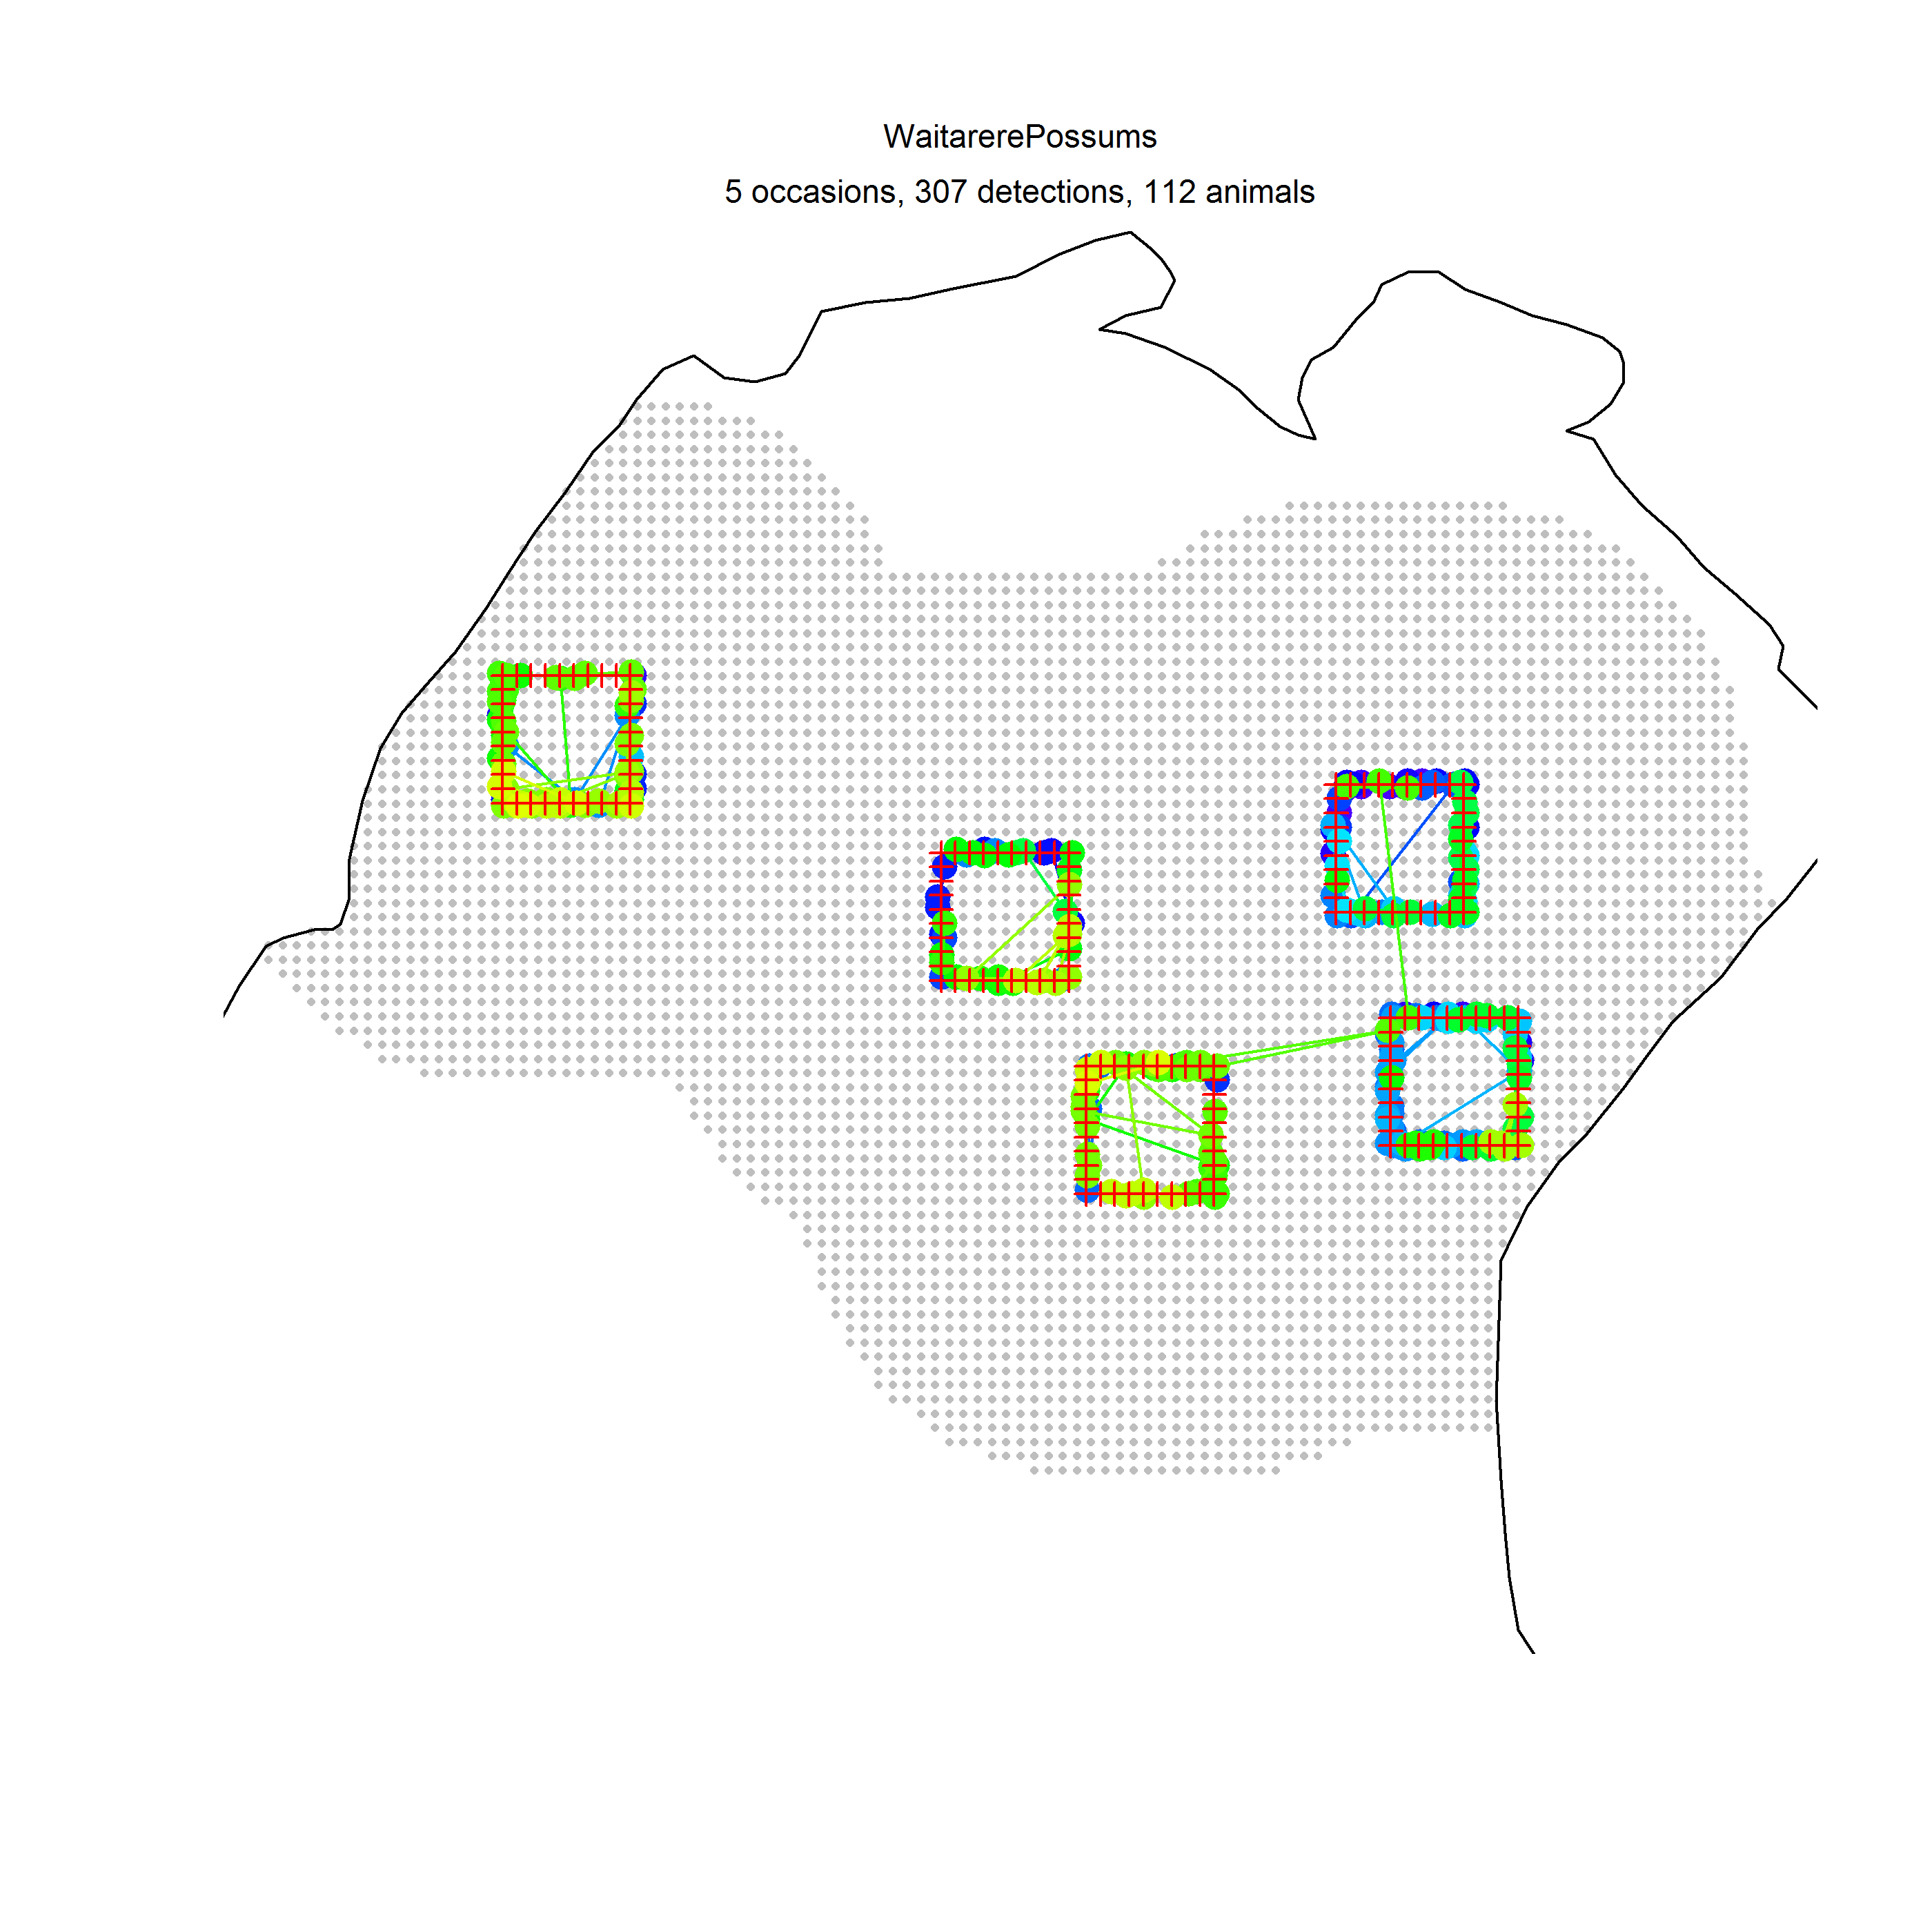
\includegraphics[width=5in,height=3.2in]{Ch5-PoisMn/figs/possum.png}
\caption{Trapping grids used in possum study from
  \citet{efford_etal:2005}, data are contained in the \R
package \mbox{\tt secr}
\citep{efford:2011}, refer to the help file \mbox{\tt ?possum} for
additional details of this study.}
\label{poisson-mn.fig.possum}
\end{figure}

The data file \mbox{\tt possumCH} contains 112 encounter histories,
and we analyzet those here although the last 8 of those are recaptures
treated as new individuals\footnote{M. Efford, personal communication}.
%Trapping produced
%46 adult females, 33 adult males, 10 immature females and 11
%immature males; sex and/or age were not recorded for 4 individuals
%(M. Coleman unpubl. data).
The encounter process is not strictly a single-catch multinomial process because,
as noted in the \mbox{\tt possum} help file
 ``One female possum was twice captured at two
sites on one day, having entered a second trap after being released;
one record in each pair was selected arbitrarily and discarded.''
which is a similar problem as we might have in bird mist net studies.
If this was a significant problem then it might be worth describing a
model fo $n_{ik} = $ the number of captures of individual $i$ during
sample $k$ to make use of all captures. By discarding the two
extra-capture events, we can satisfactorily view these data as
single-catch data, for which \mbox{\tt secr} uses the independent
multinomial likelihood (M. Efford, pers. comm.).

For our analysis we just tossed up a rectangular state-space which
doesn't account for any geographic boundaries of the suvey region, but
we note that a habitat mask is included in \secr, and we analyze the
data using that mask in Chapt. \ref{chapt.mle}.
Whether or not we use the mask is
probably immaterial as long as we understand the predictions of $N$ or
$D$ over the ocean don't mean anything biological and we probably
wouldn't report such predictions.

XXX add code here
to set up the analysis we do this.....
XXXXX

XXXX Script for doing this needs to be put in the repo XXXXXXX
Note that we define Dha in the WinBUGS script.
XXX This is fashioned after the ind. multinomial model.

{\small
\begin{verbatim}
> summary(out2)

Iterations = 501:2500
Thinning interval = 1
Number of chains = 3
Sample size per chain = 2000

1. Empirical mean and standard deviation for each variable,
   plus standard error of the mean:

             Mean        SD  Naive SE Time-series SE
D       1.541e-04 1.223e-05 1.579e-07      6.113e-07
Dha     1.541e+00 1.223e-01 1.579e-03      6.113e-03
N       2.342e+02 1.858e+01 2.399e-01      9.288e-01
alpha0 -7.380e-01 1.539e-01 1.987e-03      6.189e-03
alpha1  1.952e-04 2.052e-05 2.649e-07      1.302e-06
psi     4.686e-01 4.282e-02 5.528e-04      2.002e-03
sigma   5.082e+01 2.691e+00 3.474e-02      1.711e-01

2. Quantiles for each variable:

             2.5%        25%        50%        75%      97.5%
D       1.316e-04  1.455e-04  1.534e-04  1.619e-04  1.797e-04
Dha     1.316e+00  1.455e+00  1.534e+00  1.619e+00  1.797e+00
N       2.000e+02  2.210e+02  2.330e+02  2.460e+02  2.730e+02
alpha0 -1.043e+00 -8.411e-01 -7.387e-01 -6.368e-01 -4.308e-01
alpha1  1.565e-04  1.811e-04  1.949e-04  2.086e-04  2.379e-04
psi     3.876e-01  4.400e-01  4.675e-01  4.957e-01  5.563e-01
sigma   4.584e+01  4.896e+01  5.065e+01  5.254e+01  5.652e+01
\end{verbatim}
}

The estimated density (posterior mean) is about 1.54 possums/ha which
compares well with the estimated obtained from \secr (see
Chapt. \ref{chapt.mle} for more on the use of \secr).
To fit these data we do this (default to half-normal function)
\begin{verbatim}
secr.fit( capthist = possumCH, trace = F )
\end{verbatim}
which produces summary output like this
\begin{verbatim}
[... some output deleted ...]

Fitted (real) parameters evaluated at base levels of covariates
       link   estimate SE.estimate        lcl        ucl
D       log  1.6988930  0.17352645  1.3913904  2.0743547
g0    logit  0.1968542  0.02256272  0.1563319  0.2448321
sigma   log 51.4689114  2.59981905 46.6204139 56.8216500

[... some output deleted ...]
\end{verbatim}
There are a million reasons for potential differences some of which
we've discussed in the context of Bayesian and likelihood estimates
(Chapt. \ref{chapt.closed} sec. XXXX).
But even among likelihood estimates -- any time you run a model there
is some numerical integration going on which requires some specific
choices of how to do the integration (see
Chapt. \ref{chapt.mle}). Also \secr uses the conditional likelihood
\citep{borchers_efford:2008} which we expect to induce a slight
difference.
For now we just observe that the estimated density is certainly in the
ballpark and so too is the estimated $\sigma$.






\section{Summary and Outlook}

In this chapter we extended the basic SCR model structure to
accommodate alternative observation models, including Poisson and
multinomial observation models.
Along with the binomial model described in Chapt. \ref{chapt.scr0},
this sequence of models will accommodate the vast majority of
contemporary spatial capture-recapture problems. These models provide
the general framework for modeling the 3 main types of encounter data:
binary encounters, multinomial trials from ``multi-catch'' or
``single-catch'' \citep{efford:2004, efford:2011} trap systems, and encounter frequency
data from devices that can record multiple encounters of the same
individual at a device.

The single-catch system, as a sequence of dependent multinomial trials
(essentially a removal process operating on traps) we only did a ad
hoc analysis of this.
Figuring out the formal analysis of the single catch system would be
a nice research project for a grad student or something.
Seems like order of capture needs to be integrated into the model somehow.

There are other types of encounter models that arise in
practice. We identify a few of them here, although we neglect a
detailed development of them at the present time or, in some cases, put that off until
later chapters.
(1) Removal systems. Sometimes traps kill individuals and SCR models can handle
that. This can be viewed as a kind of open model, with mortality only, and we handle that
in Section XXXX Beth? XXXX;
(2) Trapping webs: REF XXX XXXX
would be possible to formulate trapping webs as a hierarchical model
but we haven't pursued this because trapping webs are simply not used
in practice, or their use is extremely rare.  Idea is that competition
among traps .... dividing constant density of individuals into a
variable density of traps...;
(3) Acoustic devices; What is this thing? XXXXX We need a 2 sentence
summary here... XXXX;
(4)
There are models for which
only specific summary statistics are observable
\citep{chandler_royle:2012}
which we cover in Chapts. \ref{chapt.scr-unmarked}-
\ref{chapt.partialID};
(5) We can have multiple observation methods working together as in
\citet{gopalaswamy_etal:2012} which we summarize in sec. XXXXX;
(6) In so-called search-encounter models we have slightly different
considerations -- there is an intermediate ``process'' related to
movement and so our observations.... not sure how to discuss that here.



